\section{问题三：算力约束下的资源联合优化与结构性转移}
\label{sec:problem3}

\subsection{优化模型的建立}

\subsubsection{决策变量与目标函数}

以问题二的广义标度律~\eqref{eq:p2_GSL} 为目标函数。决策变量为参数量 $N$、训练 Token 数 $D$、处理后数据质量 $Q_A$ 与领域配比 $\boldsymbol p$；预算 $C$、上下文长度 $L_{\mathrm{ctx}}$、质量成本函数 $g$ 与质量映射斜率 $s_Q$ 为外生情景变量。

\textbf{配比的处理。}由定理~\ref{thm:gsl}(4)，对任意固定 $\boldsymbol p$，Loss 可写成 $E+\Phi(N,D,Q_A)\,e^{\theta R(\boldsymbol p)}$，而三类成本都与 $\boldsymbol p$ 无关。因此联合优化可以\textbf{分两步精确求解}：
\begin{equation}
\min_{N,D,Q_A,\boldsymbol p}L=E+\Big[\min_{\boldsymbol p\in\mathcal P}e^{\theta R(\boldsymbol p)}\Big]\cdot\Big[\min_{(N,D,Q_A)\in\Omega(C)}\Phi(N,D,Q_A)\Big],
\label{eq:p3_separable}
\end{equation}
其中 $\mathcal P$ 为问题一的配比支持域~\eqref{eq:p1_opt}，$\Omega(C)$ 为预算可行域。第一步的解就是问题一的近优配比 $\boldsymbol p^\star$，\textbf{与预算无关}；第二步在 $\boldsymbol p$ 固定下优化 $(N,D,Q_A)$。由此得到一个重要推论：\textbf{最优领域配比不随预算发生结构性转移，结构性转移只可能发生在规模与质量之间}。严格地说，基线质量 $Q_0(\boldsymbol p)=\boldsymbol p^{\mathsf T}\boldsymbol q$ 也依赖配比，但 $Q_0(\boldsymbol p^\star)=0.5454$ 与 $Q_0(\boldsymbol p_{\mathrm{ref}})=0.5390$ 仅差 $0.006$；为保守起见，第二步统一取 $Q_0=0.5390$。下文先在 $\boldsymbol p_{\mathrm{ref}}$ 下求解 $(N^*,D^*,Q_A^*)$，再乘以配比因子得到 $\boldsymbol p^\star$ 下的最优 Loss。

\subsubsection{算力成本与约束}

三类开销为
\begin{equation}
C_{\mathrm{train}}=6ND,\qquad
C_Q=D\,[g(Q_A)-g(Q_0)]_+,\qquad
C_{\mathrm{attn}}=\eta NDL_{\mathrm{ctx}},\quad \eta=2\times10^{-4},
\label{eq:p3_costs}
\end{equation}
其中 $6ND$ 为训练算力的标准近似\cite{kaplan2020scaling,hoffmann2022compute}；自注意力的计算量随序列长度增长\cite{vaswani2017attention,dao2022flashattention}，在总 Token 数固定时，每个 Token 的附加开销近似正比于 $L_{\mathrm{ctx}}$。质量成本采用附录 B 给出的三类函数：
\begin{equation}
g_{\exp}(Q)=10^{7}e^{6Q},\qquad
g_{\mathrm{pow}}(Q)=5\times10^{9}Q^{4},\qquad
g_{\log}(Q)=2\times10^{9}\ln(1+10Q).
\label{eq:p3_g}
\end{equation}
三者的差异在于边际成本的形状：指数型的边际成本随质量加速上升（“越往后越贵”），幂函数型在低质量区极便宜而高质量区陡增，对数型则前期投入大、后期几乎免费。优化模型为
\begin{equation}
\begin{aligned}
\min_{N,D,Q_A}\quad & \Phi(N,D,Q_A)=A n^{-\alpha}+Bd^{-\beta}+c_Q(1-Q_{\mathrm{eff}})^{\nu_Q}\\
\text{s.t.}\quad & (6+\eta L_{\mathrm{ctx}})ND+D\,[g(Q_A)-g(Q_0)]_+\le C,\\
& N_{\min}\le N\le N_{\max},\quad D_{\min}\le D\le D_{\max},\quad Q_0\le Q_A\le Q_{\mathrm{sat}},
\end{aligned}
\label{eq:p3_model}
\end{equation}
其中 $Q_{\mathrm{sat}}=\min\{1,\ Q_0+(1-\varepsilon-Q_0)/s_Q\}$ 使有效质量不超过 1。为区分“有数据支撑的结论”与“外推结论”，设置两层可行域：严格支持域 $N\in[0.07,12]\mathrm{B}$、$D\in[10,300]\mathrm{B}$（B1/B7 的观测范围）与扩展域 $N\in[0.07,10^4]\mathrm{B}$、$D\in[0.1,3.6\times10^4]\mathrm{B}$；主结果在扩展域中求解，并对每个解标注支持状态。

\subsection{上下文长度的临界值与可行取值}

由式~\eqref{eq:p3_costs}，注意力开销与基础训练开销之比为
\begin{equation}
\frac{C_{\mathrm{attn}}}{C_{\mathrm{train}}}=\frac{\eta L_{\mathrm{ctx}}}{6},
\label{eq:p3_ratio}
\end{equation}
它与 $N,D,C$ 均无关。令其等于 1，得到两者相当的临界上下文长度
\begin{equation}
L_{\mathrm{ctx}}^{\mathrm{crit}}=\frac{6}{\eta}=\frac{6}{2\times10^{-4}}=30000\ \text{Token}.
\label{eq:p3_Lcrit}
\end{equation}
$L_{\mathrm{ctx}}$ 的可行取值依据 C7：其 45 条经核验的模型记录给出 $2048$、$4096$、$8192$、$32768$、$131072$ 五档上下文窗口，对应比值分别为 $0.068$、$0.137$、$0.273$、$1.092$、$4.369$。前三档注意力开销不足训练开销的 $30\%$，后两档已越过临界点：$32\mathrm{K}$ 时注意力开销略超训练开销，$128\mathrm{K}$ 时是训练开销的 4.4 倍。由于比值与预算无关，$L_{\mathrm{ctx}}$ 的作用等价于把单位参数—Token 的训练成本从 $6$ 放大到 $6+\eta L_{\mathrm{ctx}}$，即\textbf{有效预算}缩小为 $C/(1+\eta L_{\mathrm{ctx}}/6)$。

\subsection{模型求解}

\subsubsection{解析降维}

记 $\Delta g=[g(Q_A)-g(Q_0)]_+$，总成本可写成 $C_{\mathrm{tot}}=D\left[(6+\eta L_{\mathrm{ctx}})N+\Delta g(Q_A)\right]$。由于 $\partial\Phi/\partial D<0$，最优解必然用尽预算（或触及 $D_{\max}$），于是
\begin{equation}
D^*(N,Q_A)=\min\left\{D_{\max},\ \frac{C}{(6+\eta L_{\mathrm{ctx}})N+\Delta g(Q_A)}\right\},
\label{eq:p3_Dstar}
\end{equation}
三维约束问题化为 $(\log N,Q_A)$ 上的二维有界问题。在 $Q_A=Q_0$ 且无边界约束时，还有闭式解
\begin{equation}
n^*=\left(\frac{\alpha A}{\beta B}\right)^{\frac1{\alpha+\beta}}\overline C^{\frac{\beta}{\alpha+\beta}},\qquad d^*=\frac{\overline C}{n^*},\qquad \overline C=\frac{C}{(6+\eta L_{\mathrm{ctx}})\times10^{18}},
\label{eq:p3_closed}
\end{equation}
用作初值与正确性核对。图~\ref{fig:p3_land} 展示了 $4096$ 上下文、$10^{19}$ FLOPs 下降维后的目标景观：三种成本函数都形成一条“参数—质量”相互替代的谷地，但谷底位置截然不同——指数成本得到内点解 $Q_A^*=0.671$，幂函数成本停在下界 $Q_A^*=Q_0$，对数成本则直达上界 $Q_A^*=1$。

\begin{figure}[htbp]
\centering
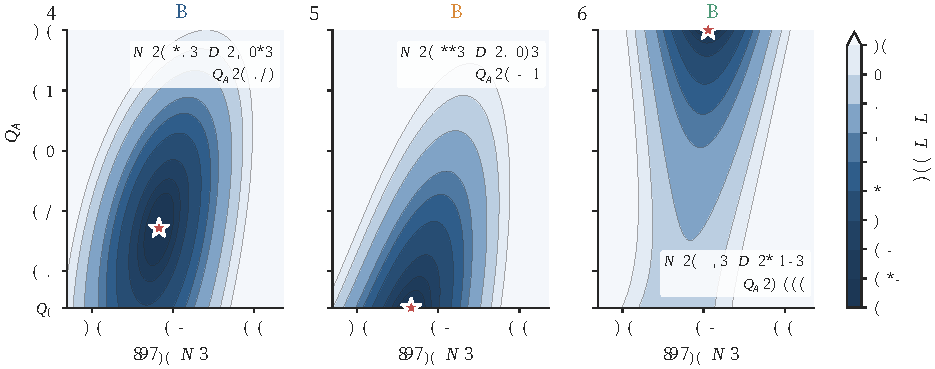
\includegraphics[width=\linewidth]{images/no3/P3_F03_三类质量成本下的低预算优化景观.pdf}
\caption{低预算（$10^{19}$ FLOPs，$L_{\mathrm{ctx}}=4096$）下三类质量成本的降维目标景观}
\label{fig:p3_land}
\end{figure}

\subsubsection{求解算法}

完整求解流程见算法~\ref{alg:p3}。粗网格保证全局覆盖，多起点 SLSQP 负责局部精化，预算追踪保证路径连续，完整三维非线性规划与加密网格用于独立核对。

\begin{algorithm}[htbp]
\caption{算力约束下的资源配置与结构转移识别}
\label{alg:p3}
\begin{algorithmic}[1]
\Require 广义标度律参数、$Q_0$、预算网格 $\mathcal C$（$10^{19}$--$10^{24}$，61 点）、上下文集合 $\mathcal L$、成本函数集合 $\mathcal G$
\Ensure 各情景最优解 $(N^*,D^*,Q_A^*)$、成本份额、活跃约束集合与转移点
\ForAll{$g\in\mathcal G$，$L_{\mathrm{ctx}}\in\mathcal L$}
  \ForAll{$C\in\mathcal C$（升序）}
    \State 在 $(\log N,Q_A)$ 粗网格上按式~\eqref{eq:p3_Dstar} 计算目标，剔除不可行点
    \State 取最优的 20 个网格点及上一预算的最优解为初值，执行 SLSQP 局部精化
    \State 对三档主预算用完整三维 NLP 与加密网格独立复核
    \State 记录成本份额、活跃约束集合 $\mathcal A(C)$ 与支持状态
  \EndFor
  \State 比较相邻预算的 $\mathcal A(C)$ 识别主要转移，二分加密至 $\Delta\log_{10}C\le0.01$
  \State 对配置弹性作分段线性拟合，识别次要转移
\EndFor
\State 500 组参数 bootstrap 传播不确定性；200 条抽样路径估计转移出现概率
\end{algorithmic}
\end{algorithm}

\subsubsection{KKT 条件与资源竞争}

设预算约束活跃、乘子为 $\mu>0$，质量上下界的乘子为 $\underline\lambda,\overline\lambda\ge0$。KKT 条件给出
\begin{equation}
\frac{-\partial\Phi/\partial N}{\partial C_{\mathrm{tot}}/\partial N}
=\frac{-\partial\Phi/\partial D}{\partial C_{\mathrm{tot}}/\partial D}
=\mu,\qquad
-\frac{\partial\Phi}{\partial Q_A}-\mu\,Dg'(Q_A)+\underline\lambda-\overline\lambda=0,
\label{eq:p3_kkt}
\end{equation}
其中 $\partial C_{\mathrm{tot}}/\partial N=(6+\eta L_{\mathrm{ctx}})D$，$\partial C_{\mathrm{tot}}/\partial D=(6+\eta L_{\mathrm{ctx}})N+\Delta g$。式~\eqref{eq:p3_kkt} 的经济含义是：\textbf{最优时每一单位算力无论投向参数、数据还是质量，带来的 Loss 降幅都相等}。据此，质量投入有三种状态：
\begin{itemize}
\item \textbf{未启动}（$Q_A^*=Q_0$，$\underline\lambda>0$）：质量的单位算力收益 $-\partial\Phi/\partial Q_A\big/(Dg'(Q_0))$ 低于规模的单位算力收益 $\mu$，全部算力用于 $N,D$；
\item \textbf{竞争}（$Q_0<Q_A^*<Q_{\mathrm{sat}}$，$\underline\lambda=\overline\lambda=0$）：三种资源的单位算力收益相等；
\item \textbf{饱和}（$Q_A^*=Q_{\mathrm{sat}}$，$\overline\lambda>0$）：质量已达上限，新增算力重新全部流向规模扩张。
\end{itemize}
预算增大时 $D$ 增大，质量的总收益 $D\cdot(-\partial\Phi/\partial Q_A)$ 与数据量成正比地放大，而规模的边际收益按幂律递减，因此质量投入必然经历“未启动 $\to$ 竞争 $\to$ 饱和”的顺序。

\subsubsection{结构性转移的数学定义与识别}

\begin{definition}[结构性转移]
固定 $(g,L_{\mathrm{ctx}},s_Q)$，记预算 $C$ 下最优解的活跃约束集合为
\begin{equation}
\begin{gathered}
\mathcal A(C)=\big\{\,c\in\mathcal K:\ c\ \text{在最优解}\ x^*(C)\ \text{处取等号}\big\},\\
\mathcal K=\{Q_A=Q_0,\ Q_A=Q_{\mathrm{sat}},\ N=N_{\min/\max},\ D=D_{\min/\max},\ C_{\mathrm{tot}}=C\}.
\end{gathered}
\label{eq:p3_active}
\end{equation}
若存在 $C^\dagger$ 使 $\mathcal A(C^{\dagger-})\neq\mathcal A(C^{\dagger+})$，称 $C^\dagger$ 为\textbf{主要结构性转移}点，此时最优策略的\textbf{类型}发生质变（如质量投入从未启动变为启动）。在 $\mathcal A(C)$ 不变的区段内，定义配置弹性
\begin{equation}
\theta_x(C)=\frac{\mathrm d\ln x^*(C)}{\mathrm d\ln C},\qquad x\in\{N,\ D,\ Q_A-Q_0\},
\label{eq:p3_elasticity}
\end{equation}
若 $\theta_x$ 在某点发生跳变（分段线性拟合相对单一直线的 BIC 改善 $\ge10$\cite{schwarz1978estimating}，且两侧斜率差 $\ge0.15$），称为\textbf{次要结构性转移}，此时策略类型不变但资源增长的主次关系改变。只有在至少 $70\%$ 的参数抽样路径中都出现的转移才认定为\textbf{稳定转移}。
\end{definition}

识别方法：在 61 个对数等距预算点上追踪 $\mathcal A(C)$，发现变化后二分加密至 $\log_{10}C$ 区间宽度 $\le0.01$；次要转移在活跃集不变的区段内用分段回归定位。

\subsection{求解结果}

\subsubsection{三档预算下的最优配置}

以 $L_{\mathrm{ctx}}=4096$、$s_Q=1$ 为主情景，三档预算的最优配置见表~\ref{tab:p3_main}。其中 $L^*_{\mathrm{ref}}$ 为参考配比下的最优 Loss，$L^*_{\star}$ 为采用近优配比 $\boldsymbol p^\star$ 后的最优 Loss（由式~\eqref{eq:p3_separable}，$L^*_\star=E+(L^*_{\mathrm{ref}}-E)\times0.824$）。

\begin{table}[htbp]
\centering
\small
\caption{$L_{\mathrm{ctx}}=4096$ 下三档预算的最优资源配置}
\label{tab:p3_main}
\setlength{\tabcolsep}{4pt}
\begin{tabular}{llrrcccccl}
\toprule
成本 & 预算/FLOPs & $N^*$/B & $D^*$/B & $D^*/N^*$ & $Q_A^*$ & 质量份额 & $L^*_{\mathrm{ref}}$ & $L^*_\star$ & 支持状态 \\
\midrule
指数 & $10^{19}$ & 0.259 & 4.82 & 19 & 0.671 & 14.8\% & 3.1690 & 2.9082 & 单分量外推 \\
 & $10^{22}$ & 5.449 & 244.3 & 45 & 1.000 & 9.2\% & 2.1549 & 2.0729 & 观测支持 \\
 & $10^{24}$ & 39.58 & 3653.8 & 92 & 1.000 & 1.4\% & 1.9160 & 1.8761 & 外推 \\
\midrule
幂函数 & $10^{19}$ & 0.215 & 6.81 & 32 & 0.539 & 0.0\% & 3.1796 & 2.9170 & 单分量外推 \\
 & $10^{22}$ & 5.558 & 235.4 & 42 & 1.000 & 10.8\% & 2.1563 & 2.0741 & 观测支持 \\
 & $10^{24}$ & 39.71 & 3631.3 & 91 & 1.000 & 1.7\% & 1.9161 & 1.8762 & 外推 \\
\midrule
对数 & $10^{19}$ & 0.337 & 2.95 & 9 & 1.000 & 32.1\% & 3.1181 & 2.8663 & 单分量外推 \\
 & $10^{22}$ & 5.048 & 281.6 & 56 & 1.000 & 3.1\% & 2.1498 & 2.0687 & 观测支持 \\
 & $10^{24}$ & 39.13 & 3732.4 & 95 & 1.000 & 0.4\% & 1.9157 & 1.8759 & 外推 \\
\bottomrule
\end{tabular}
\end{table}

\textbf{成本函数的影响集中在低预算。}在 $10^{19}$ FLOPs，三种成本函数给出三种截然不同的策略：对数成本前期昂贵、后期平坦，一旦投入就直接做到最高质量，用 $32.1\%$ 的预算提质，同时把数据量压到 $2.95\mathrm{B}$；指数成本选择中间质量 $0.671$；幂函数成本则完全不提质，把算力全部投给规模。到 $10^{22}$ 与 $10^{24}$ FLOPs，三种成本函数都达到质量上限，最优参数量、数据量与 Loss 趋于一致（$10^{24}$ 时 Loss 差异小于 $5\times10^{-4}$），\textbf{成本函数的形状不再重要}。

\textbf{质量在高预算下是“必选项”，而其算力占比很小。}$10^{22}$ FLOPs 时，把质量提升到上限只占用 $3.1\%$--$10.8\%$ 的预算，到 $10^{24}$ FLOPs 更降至 $0.4\%$--$1.7\%$。这是因为质量成本按单位 Token 计费，而训练成本按“参数 × Token”计费，模型越大，质量处理的相对成本越低——这与问题二“规模越大、质量越值钱”的结论相互印证。

\textbf{数据—参数比随预算上升。}$D^*/N^*$ 从 $10^{22}$ 的 42--56 升至 $10^{24}$ 的 91--95，显著高于 Chinchilla 经验值 20\cite{hoffmann2022compute}。原因是本文 B1 拟合的 $\alpha=0.340>\beta=0.280$：参数项衰减更快，最优策略更偏向数据，且 $N^*\propto C^{0.452}$、$D^*\propto C^{0.548}$ 使数据—参数比随预算按 $C^{0.097}$ 增长。

\textbf{配比带来与预算无关的比例收益。}采用 $\boldsymbol p^\star$ 使可约损失在所有预算下都降低 $17.6\%$：Loss 在 $10^{19}$、$10^{22}$、$10^{24}$ FLOPs 下分别降低约 $0.26$、$0.08$、$0.04$。按 $R(\boldsymbol p^\star)$ 的 95\% 区间，$10^{22}$ FLOPs 下的 Loss 变化量在 $[-0.121,\ +0.004]$ 之间（最多降低 $0.121$，最坏升高 $0.004$）。

\textbf{领域 Token 分配。}最优总 Token 数按 $D_i=p_iD^*$ 分解到 17 个领域。以指数成本、$10^{22}$ FLOPs（$D^*=244.3\mathrm{B}$）为例，采用 $\boldsymbol p^\star$ 时专利背景、生医摘要、技术问答、议会文本分别分配 $59.1$、$46.2$、$36.4$、$25.3\mathrm{B}$ Token，学术论文、代码、法律、生物医学全文不再分配；若出于稳健考虑采用 $\boldsymbol p_{\mathrm{ref}}$，则各领域在 $0.5$--$29.2\mathrm{B}$ 之间较为均衡地分配。完整分配表见支撑材料。

\subsubsection{连续预算路径与结构性转移}

图~\ref{fig:p3_path} 给出 $10^{19}$--$10^{24}$ FLOPs 的连续最优路径，图~\ref{fig:p3_share} 给出对应的算力份额。通过稳定性检验的结构性转移见表~\ref{tab:p3_trans}。

\begin{figure}[htbp]
\centering
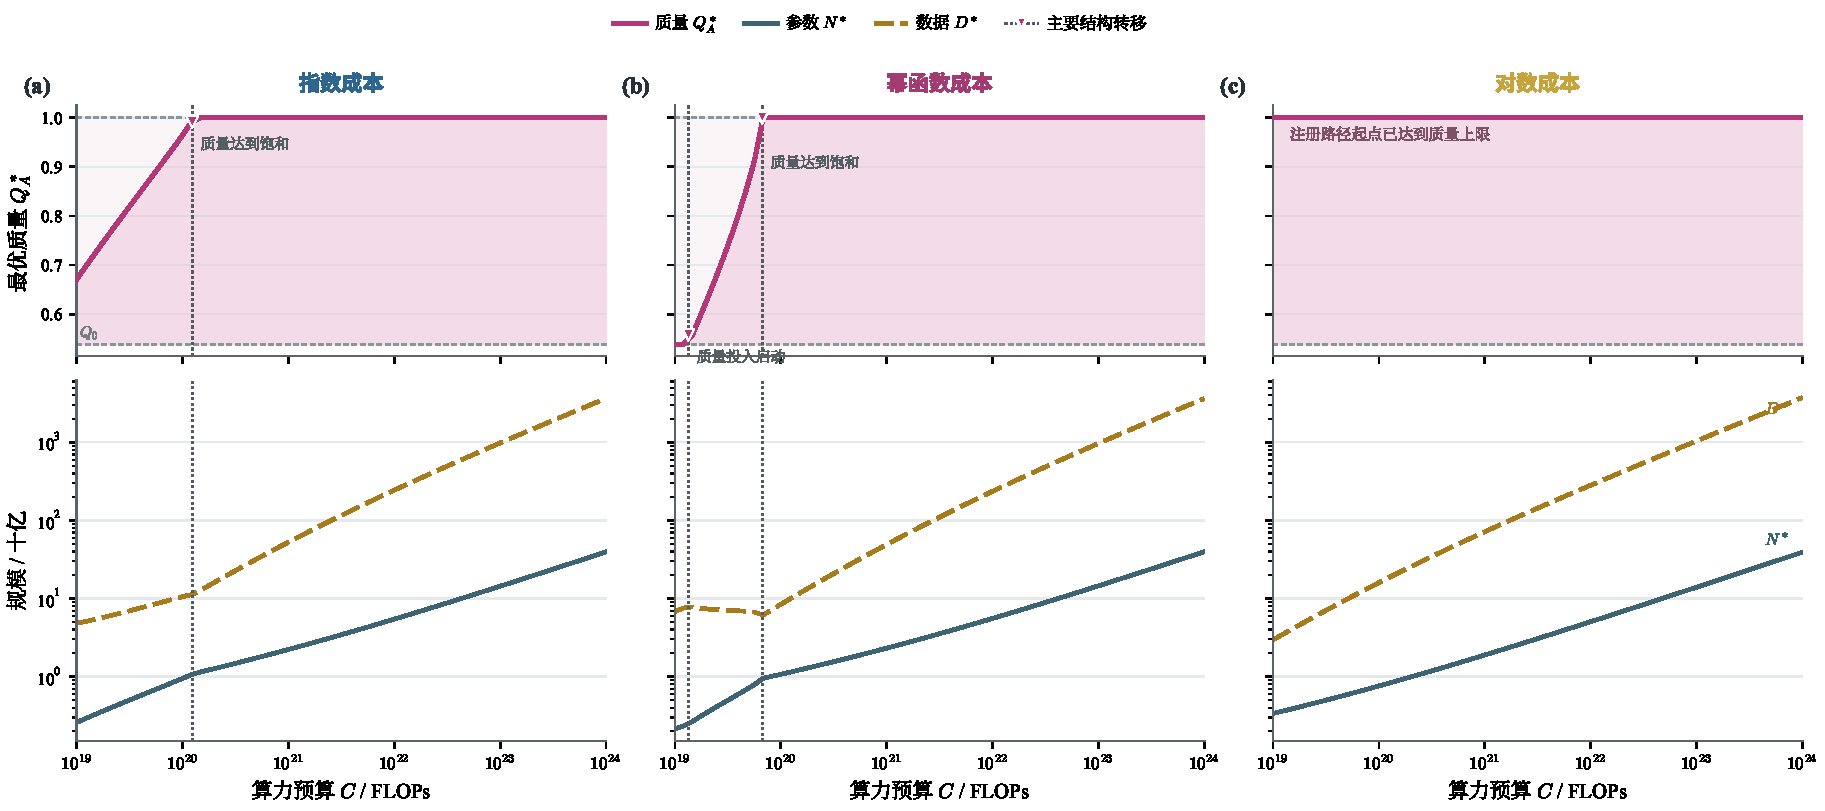
\includegraphics[width=\linewidth]{images/no3/P3_F07_最优配置路径与结构转移.pdf}
\caption{$L_{\mathrm{ctx}}=4096$ 下最优质量（a）、参数量（b）与数据量（c）随预算的变化}
\label{fig:p3_path}
\end{figure}

\begin{figure}[htbp]
\centering
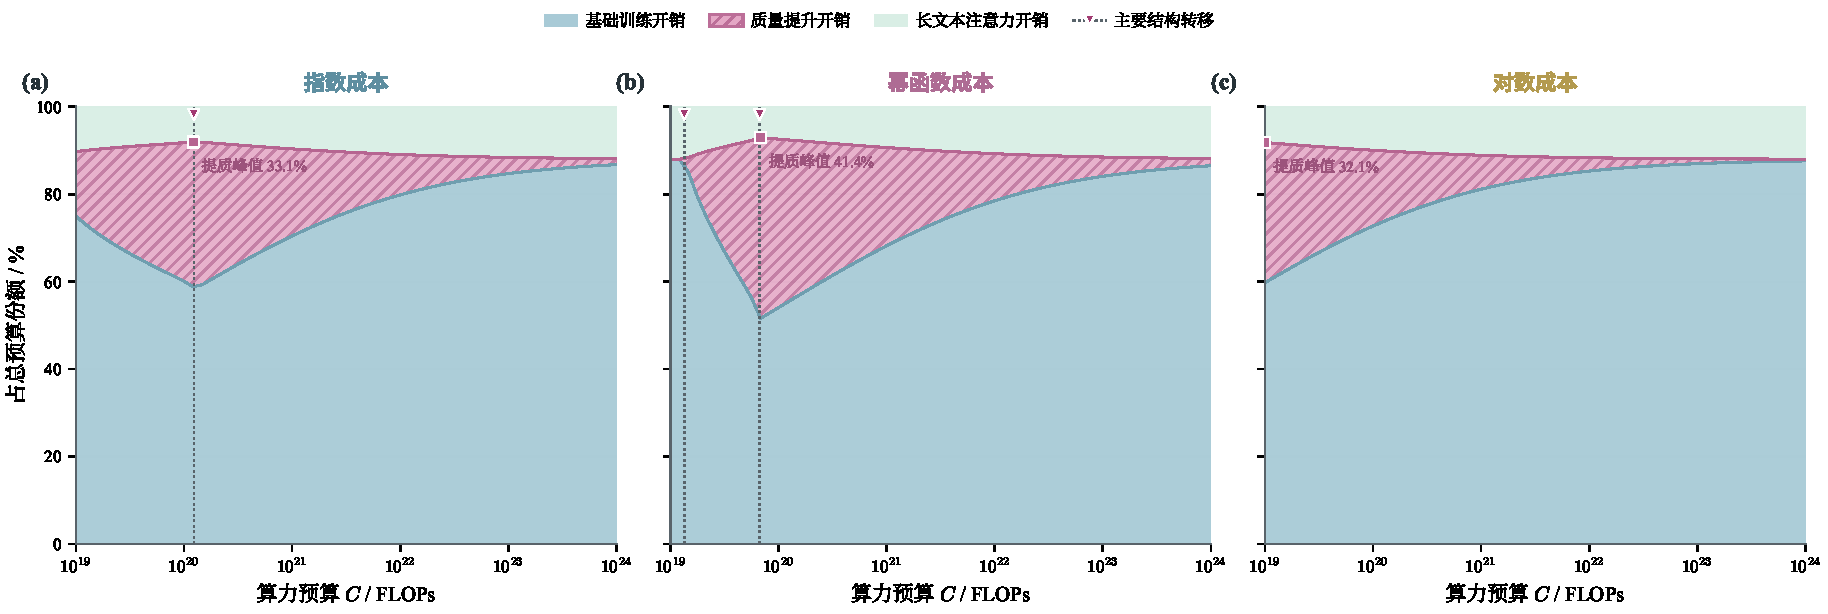
\includegraphics[width=\linewidth]{images/no3/P3_F01_预算约束下的边际资源竞争机制.pdf}
\caption{$L_{\mathrm{ctx}}=4096$ 下三类算力开销的份额随预算的变化}
\label{fig:p3_share}
\end{figure}

\begin{table}[htbp]
\centering
\small
\caption{$L_{\mathrm{ctx}}=4096$ 下的稳定结构性转移}
\label{tab:p3_trans}
\setlength{\tabcolsep}{4pt}
\begin{tabular}{lllccc}
\toprule
成本 & 类型 & 转移事件 & 临界预算/FLOPs & 95\% 区间（$\log_{10}C$） & 出现概率 \\
\midrule
幂函数 & 主要 & 质量投入启动（$Q_0$ 下界失效） & $1.34\times10^{19}$ & [19.04, 19.21] & 1.00 \\
 & 次要 & 质量增量弹性断点 & $4.22\times10^{19}$ & — & 1.00 \\
 & 主要 & 质量达到饱和（$Q_{\mathrm{sat}}$ 上界激活） & $6.69\times10^{19}$ & [19.63, 20.38] & 1.00 \\
 & 次要 & 参数量、数据量弹性断点 & $1.10\times10^{20}$ & — & 1.00 \\
\midrule
指数 & 次要 & 质量增量弹性断点 & $9.09\times10^{19}$ & — & 1.00 \\
 & 主要 & 质量达到饱和 & $1.23\times10^{20}$ & [19.79, 20.63] & 1.00 \\
 & 次要 & 数据量弹性断点 & $2.37\times10^{20}$ & — & 1.00 \\
\midrule
对数 & — & 起点即饱和，无新转移 & — & — & — \\
\bottomrule
\end{tabular}
\end{table}

结果显示了清晰的\textbf{三阶段结构性转移}，以幂函数成本最为完整：
\begin{enumerate}
\item \textbf{规模优先期}（$C<1.34\times10^{19}$）：质量投入未启动，全部算力用于参数与数据；
\item \textbf{质量—规模竞争期}（$1.34\times10^{19}\le C<6.69\times10^{19}$）：质量投入启动并快速上升，质量份额峰值达 $41.4\%$；这一阶段数据量几乎停滞在 $6$--$8\mathrm{B}$，新增算力主要在参数与质量之间分配；
\item \textbf{质量饱和、规模重新主导期}（$C\ge6.69\times10^{19}$）：质量达到上限，质量份额被持续增长的训练成本稀释（$10^{24}$ 时降至 $0.4\%$--$1.7\%$，基础训练份额回升至 $87\%$ 左右），$N^*$、$D^*$ 恢复幂律增长。
\end{enumerate}
指数成本在 $10^{19}$ 时已处于竞争期，于 $1.23\times10^{20}$ 饱和，质量份额峰值 $33.1\%$；对数成本在整个区间都处于饱和期。这与题目“收入低时先顾温饱、收入高时追求品质”的类比完全一致：\textbf{低预算先保规模，中等预算质量与规模竞争，高预算质量成为标配而规模重新成为主要增长方向}。

图~\ref{fig:p3_trans} 给出各转移预算的 bootstrap 分布。所有 8 个稳定转移的出现概率均为 1；主要转移的定位极为精确（幂函数质量启动的 95\% 区间仅为 $\log_{10}C\in[19.04,19.21]$），饱和点的不确定性稍大，主要来自质量参数 $c_Q,\nu_Q$ 的估计误差。

\begin{figure}[htbp]
\centering
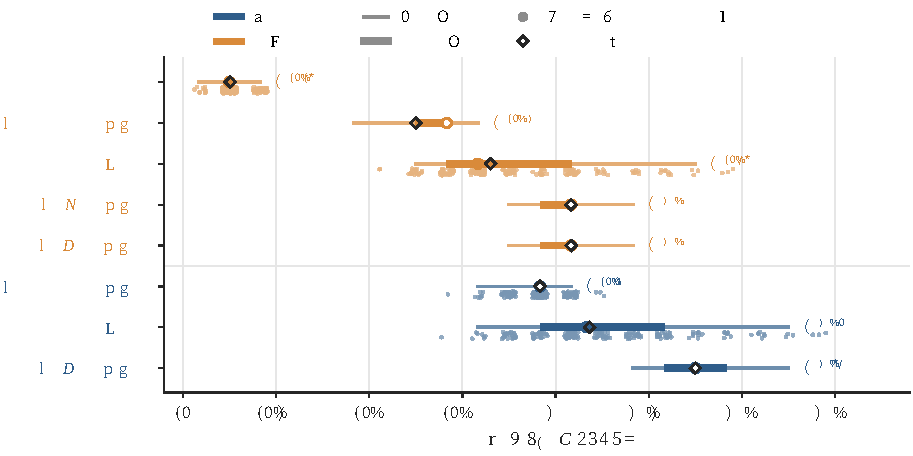
\includegraphics[width=\linewidth]{images/no3/P3_F05_稳定结构转移的区间估计.pdf}
\caption{稳定结构性转移点的 bootstrap 区间估计}
\label{fig:p3_trans}
\end{figure}

\subsubsection{上下文长度的敏感性}

在 C7 的五档可行上下文上重新求解，最优 Loss 相对 $2048$ 上下文的增量见图~\ref{fig:p3_ctx}，最优配置的变化见图~\ref{fig:p3_ctxcfg}。

\begin{figure}[htbp]
\centering
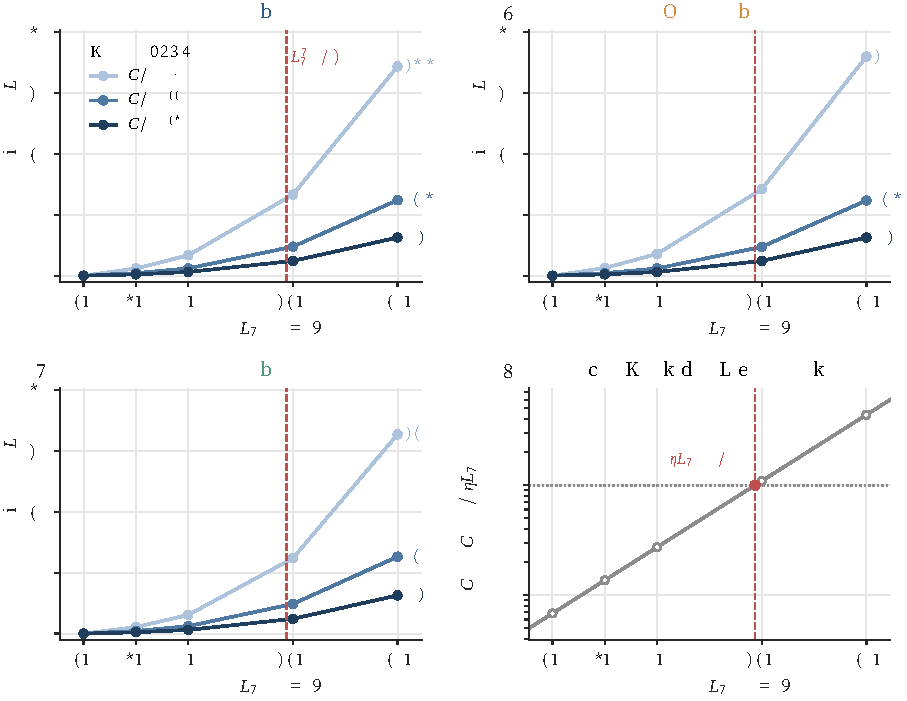
\includegraphics[width=\linewidth]{images/no3/P3_F02_上下文成本临界与最优损失惩罚.pdf}
\caption{上下文长度引起的最优 Loss 增量（a--c）与注意力/训练开销比（d）}
\label{fig:p3_ctx}
\end{figure}

\begin{figure}[htbp]
\centering
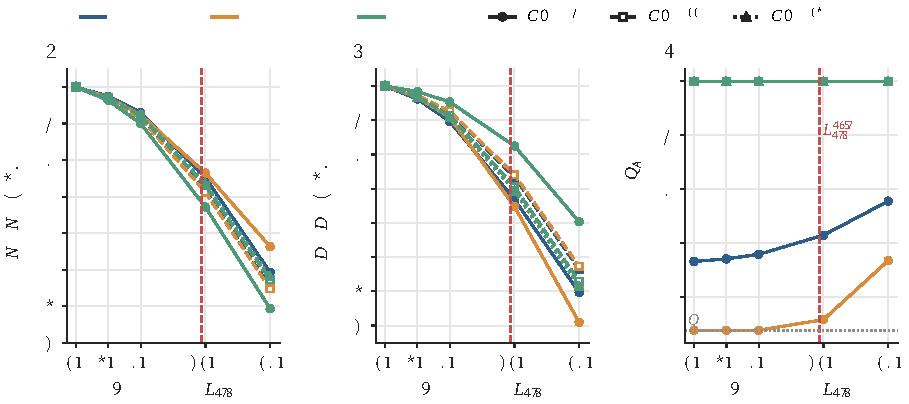
\includegraphics[width=\linewidth]{images/no3/P3_F04_上下文长度对最优配置的影响.pdf}
\caption{上下文长度对最优参数量（a）、数据量（b）与质量（c）的影响}
\label{fig:p3_ctxcfg}
\end{figure}

\begin{enumerate}
\item \textbf{临界点前后影响截然不同。}在 $L_{\mathrm{ctx}}\le8192$ 时，Loss 增量在低预算下不超过 $0.036$、在 $10^{22}$ FLOPs 以上不超过 $0.012$；越过 $30000$ 后惩罚迅速扩大——$32768$ 上下文下 $10^{19}$ FLOPs 的增量已达 $0.12$--$0.14$，$131072$ 上下文下，$10^{19}$、$10^{22}$、$10^{24}$ FLOPs 的 $100\Delta L^*$ 分别为 $32.7$--$36.0$、$12.4$--$12.6$ 和 $6.3$。\textbf{预算越低，长上下文越“奢侈”}，高预算能够通过扩大规模部分吸收这一开销。
\item \textbf{长上下文主要挤压数据量。}$131072$ 上下文下 $N^*$ 降至 $2048$ 基准的 $39\%$--$56\%$，$D^*$ 降至 $31\%$--$60\%$。低预算幂函数成本下 $D^*$ 降幅最大（至 $31\%$），同时 $Q_A^*$ 由 $0.539$ 升至 $0.668$；指数成本下 $Q_A^*$ 由 $0.666$ 升至 $0.778$——\textbf{当规模变贵时，最优策略用质量替代规模}。
\item \textbf{上下文不改变转移机制。}$L_{\mathrm{ctx}}$ 只改变有效预算，三阶段结构性转移在各档上下文下依然存在，只是转移点随有效预算缩小而向高预算方向平移。
\end{enumerate}

\subsection{模型检验与敏感性分析}

\subsubsection{数值验证}

对全部中心解逐项回代：约束违反量最大 $4.1\times10^{-16}$；二维降维解与完整三维 NLP 的相对 Loss 差最大 $4.4\times10^{-14}$；与加密网格的相对差 $2.1\times10^{-16}$；领域 Token 求和误差 $1.9\times10^{-16}$；同种子重复运行结果完全一致。图~\ref{fig:p3_ms} 以质量处于内点、局部最优风险最大的“指数成本、$10^{19}$ FLOPs”情景为例：20 个网格起点全部在 6--11 次迭代内收敛到同一最优解，最终相对 Loss 差在 $1.5\times10^{-13}$ 以内。此外，全部中心解均满足“预算增大 Loss 不增”“上下文增长 Loss 不降”等单调性检验。

\begin{figure}[htbp]
\centering
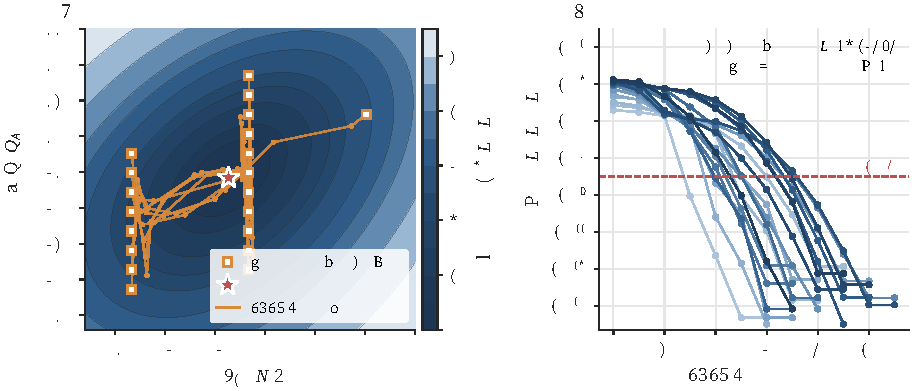
\includegraphics[width=\linewidth]{images/no3/P3_F08_多起点寻优过程与收敛验证.pdf}
\caption{多起点寻优轨迹（a）与相对 Loss 差的收敛过程（b）}
\label{fig:p3_ms}
\end{figure}

\subsubsection{参数不确定性与关键假设敏感性}

用问题二的 500 组联合 bootstrap 参数重新求解，$10^{22}$ 与 $10^{24}$ FLOPs 下最优 Loss 的 95\% 区间宽度不超过 $1.2\times10^{-4}$；$10^{19}$ FLOPs 下宽度约 $0.03$（幂函数成本最宽），主要来自质量参数的不确定性。关键假设的敏感性（共 234 个情景）见图~\ref{fig:p3_sens}：
\begin{itemize}
\item \textbf{质量映射斜率 $s_Q$} 影响最大：$s_Q=0.5$ 使 $10^{22}$、$10^{24}$ FLOPs 的 Loss 上升 $0.085$，因为此时质量提升只能部分传导到有效质量；
\item \textbf{质量成本幅度与形状}的 $\pm20\%$ 扰动只影响低预算（最大 $0.053$），高预算下几乎无影响；
\item \textbf{注意力系数 $\eta$} 的 $\pm20\%$ 扰动影响不超过 $0.005$；
\item \textbf{严格支持域}使 $10^{24}$ FLOPs 的 Loss 上升约 $0.177$，这是因为最优规模远超观测范围、被边界截断，说明高预算结论本质上依赖标度律外推。
\end{itemize}

\begin{figure}[htbp]
\centering
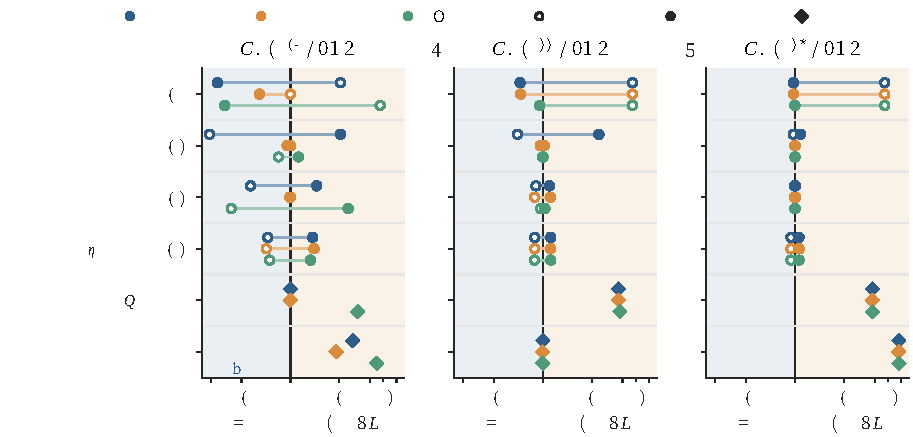
\includegraphics[width=\linewidth]{images/no3/P3_F06_关键假设的敏感性分析.pdf}
\caption{$L_{\mathrm{ctx}}=4096$ 下关键假设对最优 Loss 的影响（$100\Delta L^*$）}
\label{fig:p3_sens}
\end{figure}

\subsection{问题三小结}

\begin{conclusionbox}
\textbf{问题三主要结论}
\begin{enumerate}
\item 由广义标度律的乘性配比结构证明了配比与规模—质量决策的可分性：最优配比 $\boldsymbol p^\star$ 与预算无关，可使所有预算下的可约损失降低约 $17.6\%$。
\item 注意力与训练开销相当的临界上下文长度为 $L_{\mathrm{ctx}}^{\mathrm{crit}}=6/\eta$，即 $30000$ Token；C7 的 $32\mathrm{K}$、$128\mathrm{K}$ 两档已越过临界点，$128\mathrm{K}$ 上下文在 $10^{19}$ FLOPs 下使最优 Loss 上升约 $0.33$--$0.36$。
\item 以 $4096$ 上下文、指数成本为例，三档预算的最优参数量分别为 $0.26$、$5.45$、$39.6\mathrm{B}$，最优 Token 数分别为 $4.8$、$244$、$3654\mathrm{B}$，最优质量分别为 $0.671$、$1.0$、$1.0$；最优 Loss 为 $3.169$、$2.155$、$1.916$，采用 $\boldsymbol p^\star$ 后为 $2.908$、$2.073$、$1.876$。
\item 以 KKT 活跃约束集合的变化定义结构性转移，识别出“规模优先 $\to$ 质量—规模竞争 $\to$ 质量饱和、规模主导”的三阶段转移；幂函数成本下两个主要转移点分别为 $1.34\times10^{19}$ FLOPs 与 $6.69\times10^{19}$ FLOPs，出现概率均为 1。成本函数形状只在低预算下重要。
\end{enumerate}
\end{conclusionbox}
